\pdfbookmark[1]{Simulations}{simulations}
    % - How we are inspired from other articles of how we compute the Hamiltonian - Plot the fluxonium potential
	% - Simulate numerical in the flux-basis and get the energies and the eigenstates
	% - Then we simulate it in different cases and say something about what E_J, E_C and gamma etc. should be 
	% - (simulate the gates of fluxonium and say how the energy is going to be). 
Here in the simulation part, it is something we do before making a design because there are many values we need to know what approximate should be like how to design the parameters of the resonators in order to get the right impedance, or what the values of the different components in the fluxonium should be or the legnth of the resonators to estimate a frequency there is within our length but does not go into the TWPA frequency and neither. or how many jj there should be in the array (also with "rightsizing array  of josephson junction article". )

\chapter{Simulation Fluxonium spectrum in python}
	\section{Simulating energy eigenvalues and wave function using numerical analysis of the Hamiltonian}
    In order to simulate the energy levels of a Fluxonium qubit (eq. \ref{eq:hamiltonian_fluxonium}), we start by changing to the flux basis which allows us to numerical write up the magnetic flux as a diagonal matrix. The first term in the Hamiltonian is corresponding to the capacitor (kinetic energy). In the flux basis, it is proportional to the derivative of the flux. The relationship between the flux, $\hat{n}$ and charge is given by \cite{Aumann2022}. 
        \begin{equation}
            \begin{aligned}
                 \hat{n} =  \frac{\hat{q}}{2e} = -i \frac{\partial}{\partial \phi} \\
                \hat{n}^{2} = -\frac{\partial}{\partial \phi^{2}}  = \frac{\hat{q}^{2}}{4e^2}
            \end{aligned}
        \end{equation}
        We will take $\hat{q}$ and the $\hat{q}^2$ to be: \cite{Aumann2022}: 
        \begin{equation}
            \hat{q} =\frac{-\mathrm{i} \hbar}{2 \delta}\left(\begin{array}{cccc}
            0 & 1 & & \\
            -1 & 0 & 1 & \\
            & & \ddots & \\
            & & -1 & 0
            \end{array}\right) 
            ,
            \hat{q}^2 = \frac{-\hbar^2}{\delta^2}\left(\begin{array}{cccc}
            -2 & 1 & & \\
            1 & -2 & 1 & \\
            & & \ddots & \\
            & & 1 & -2
            \end{array}\right)
        \end{equation}
    The phase operator is diagonal in the flux basis and is given by \cite{Aumann2022}:
    \begin{equation}
        \hat{\phi} \rightarrow \frac{2\pi}{\Phi_0} \left(\begin{array}{cccc}
        -\Phi_{\max } & & & \\
        & -\Phi_{\max }+\delta & & \\
        & & \ddots & \\
        & & & \Phi_{\max }
        \end{array}\right)
    \end{equation}
    The Energy spectrum is found using the following code: 
    \begin{lstlisting}[language =Python, caption=Python example]
# Define the hamiltonian for fluxonium:
    def hamiltonian(E_J,E_L,E_C,phi_ext,N,phi):
    # make our matrix phi
        Phi = np.zeros((N,N))
        for i in range(N):
            Phi[i][i]= phi[i]
    # q^2 approximated: 
    a = np.ones((1, N-1))[0]
    b = np.ones((1,N))[0]
    q_2 = np.dot(( np.diag(-2*b,0) + np.diag(a, -1) + np.diag(a, 1)), (-(1))/(delta**2))

    # Conductor term: kinetic energy
    C = np.dot(4*E_C,q_2)
    
    # JJ term: should be a positive diagonal matrix. 
    JJ = np.zeros((N,N))
    for i in range(N):
        JJ[i][i] = E_J*np.cos(Phi[i][i]-phi_ext)

    # Inductor term: positiv diagonal matrix.
    inductor = np.zeros((N,N))
    for i in range(N):
        inductor[i][i] = 1/2*E_L*(Phi[i][i])**2

    # Define the Hamiltonian.
    Hamiltonian = C - JJ + inductor
    
    # calculating the eigenvalues and eigenenergies in order.
    eig_vals, eig_vec = sp.linalg.eigh(Hamiltonian)  
    
    # returns the eigenvalues and eigenenergies eig_vals
    return eig_vals,eig_vec
    \end{lstlisting}
    Here the delta is the difference between 2 values of phi, so the pressision, in this case it is: 
    \begin{lstlisting}[language = Python]
        phi = np.linspace(-3*np.pi, 3*np.pi, N)
        # delta = 0.1885
    \end{lstlisting}
    The first 5 energy levels are plotted along with the Fluxonium potential defined as: 
    \begin{lstlisting}[language=Python]
    def fluxonium_potential_transformation(E_J,E_L,phi,phi_ext):
        return -E_J*np.cos(phi-phi_ext)+ 1/2*E_L*((phi)**2)
    \end{lstlisting} 
    Further some sliders were added in order to manipulate $E_C = 4$, $E_J = 1$, and $E_L = 1$. 
\newpage
    \begin{lstlisting}[language = Python]
# Make horizontal sliders to control the phi_ext.
    ax_phi_ext = fig.add_axes([0.1, 0.2, 0.7, 0.04])
    phi_ext_slider = Slider(
        ax=ax_phi_ext,
        label='\u03C6_ext',
        valmin=-2*np.pi,
        valmax=2*np.pi,
        valinit=init_phi_ext,)

# Make horizontal sliders to control the Josephson energy.
    ax_E_J = fig.add_axes([0.1, 0.15, 0.7, 0.04])
    E_J_slider = Slider(
        ax=ax_E_J,
        label='E_J[GHz]',
        valmin=-20.,
        valmax=20,
        valinit=init_E_J,)

# Make horizontal sliders to control the induction energy.
    ax_E_L = fig.add_axes([0.1, 0.1, 0.7, 0.04])
    E_L_slider = Slider(
        ax=ax_E_L,
        label='E_L[GHz]',
        valmin=-20.,
        valmax=20,
        valinit=init_E_L,)

# Make horizontal sliders to control the capacitor energy.
    ax_E_C = fig.add_axes([0.1, 0.05, 0.7, 0.04])
    E_C_slider = Slider(
        ax=ax_E_C,
        label='E_C[GHz]',
        valmin=-20.,
        valmax=20,
        valinit=init_E_C,)
    \end{lstlisting}
    The sliders are updated by the following code: 
    \begin{lstlisting}[language = Python]
# The function to be called anytime a slider's value changes
    def update(val):
        line.set_ydata(fluxonium_potential_transformation(E_J_slider.val, E_L_slider.val,phi, phi_ext_slider.val))
        eig_vals, eig_vec = hamiltonian(E_J_slider.val,E_L_slider.val, E_C_slider.val,phi_ext_slider.val,N, phi)
        for x in range(0, 5):
            lines["line{0}".format(x)].set_ydata(10*eig_vec.T[x]+eig_vals[x])
    phi_ext_slider.val))
        fig.canvas.draw_idle()
# Update the sliders
    phi_ext_slider.on_changed(update)
    E_J_slider.on_changed(update)
    E_L_slider.on_changed(update)
    E_C_slider.on_changed(update)    
    \end{lstlisting}
    The python plot can be seen in fig. \ref{fig:Energy_Fluxonium}. The figure shows a snapshot of our simulation of the Fluxonium energy spectrum as a function of phase, $\phi$. The parameters shown are inspired by the article \textit{Blueprint for a High-Performance Fluxonium Quantum Processor} \cite{Nguyen2022}. The external flux are $\phi_{ext} = \pi$, the capacitor energy, $E_C= 1$, the Jospehson energy, $E_J = 4$ and the inductance energy, $E_L = 1$ values. The potential is plotted in the background in order to better visioalize the energy levels: 
    \begin{lstlisting}[language = Python]
# # plot the potential as a function of the psi
# Generate N numbers between -pi and pi
    phi = np.linspace(-3*np.pi, 3*np.pi, N)
    
# define the fluxonium potential with a coordinate transformation
    def fluxonium_potential_transformation(E_J,E_L,phi,phi_ext):
        return -E_J*np.cos(phi-phi_ext)+ 1/2*E_L*((phi)**2)
    
# Eigenstates does not have any unit - therefore we add the eigenenergies
# we also plot the eigenstate squared becuase thet it the probability distribution. 
    line, = ax.plot(phi, fluxonium_potential_transformation(init_E_J, init_E_L,phi, init_phi_ext))
    \end{lstlisting}
    Changing the external flux, $\phi_{ext}$, changes the energy spacing between the two first states. They are minimized when  $\phi_{ext} = \pm \pi$. Therefore, we set $\phi_{ext} = \pi$ which is the most used value among other seen in \cite{Nguyen2022}. This is said to be the flux degeneracy point, which gives the maximum coherence time to the system \cite{Krantz2019}.  
    \begin{figure}
        \centering
        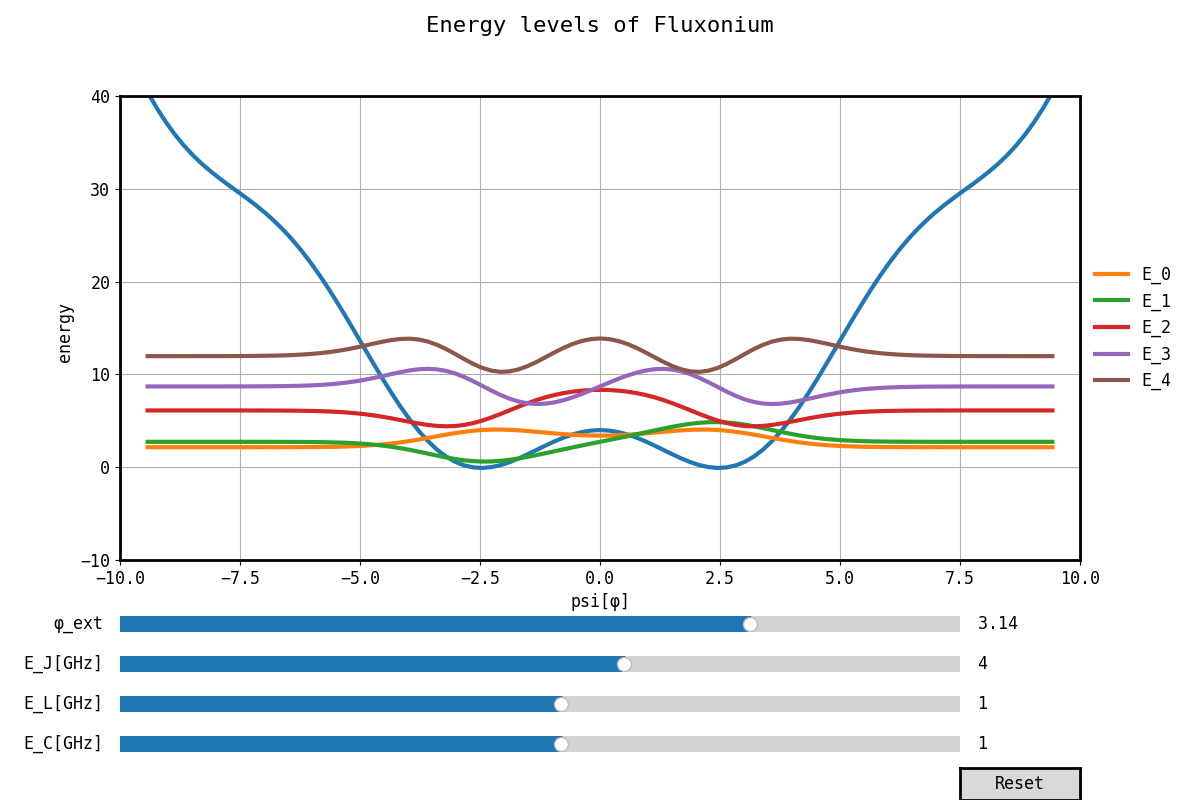
\includegraphics[width = 13.5cm]{Images/Wavefunctions_and_eigenstates_Fluxonium.png}
        \caption[Energy diagram of a Fluxonium qubit]{\textbf{Energy diagram of a Fluxonium qubit:} Snapshot of Fluxonium energy spectrum simulation as a function of phase, $\phi$. The external flux are $\phi_{ext} = \pi$, the capacitor energy, $E_C= 1$, the Jospehson energy, $E_J = 4$ and the inductance energy, $E_L = 1$ values.}
        \label{fig:Energy_Fluxonium}
    \end{figure}
    Changing the capacitor energy, $E_C$ is equivalent to giving the cooper pairs more kinetic energy. This will increase the spacing between all the energy-levels. Having a large value of $E_C$ can be good because it makes a large anharmonicity between level 01 and 21. However, it should not be too large as it will separate the two first levels too much. 
    \newline
    \newline
    The last thing we will look at, is the ratio between $E_J$ and $E_L$. The larger the difference between $E_J$ and $E_L$, the larger the anharmonicity between $\omega_{01}$ and $\omega_{12}$. At first glance, this is what we wish to obtain, but when plotting the energy levels with large ratio between $E_J$ and $E_L$ the potential will have a huge energy potential between the two first levels as seen in fig. \ref{fig:Large_ratio_EJ_EL}. The large energy potential is highlighted with a black line. The probability to excite to higher energy levels than the two first is more probable for too large ratios between $E_J$ and $E_L$ which should therefore be avoided. 
    \begin{figure}
        \centering
        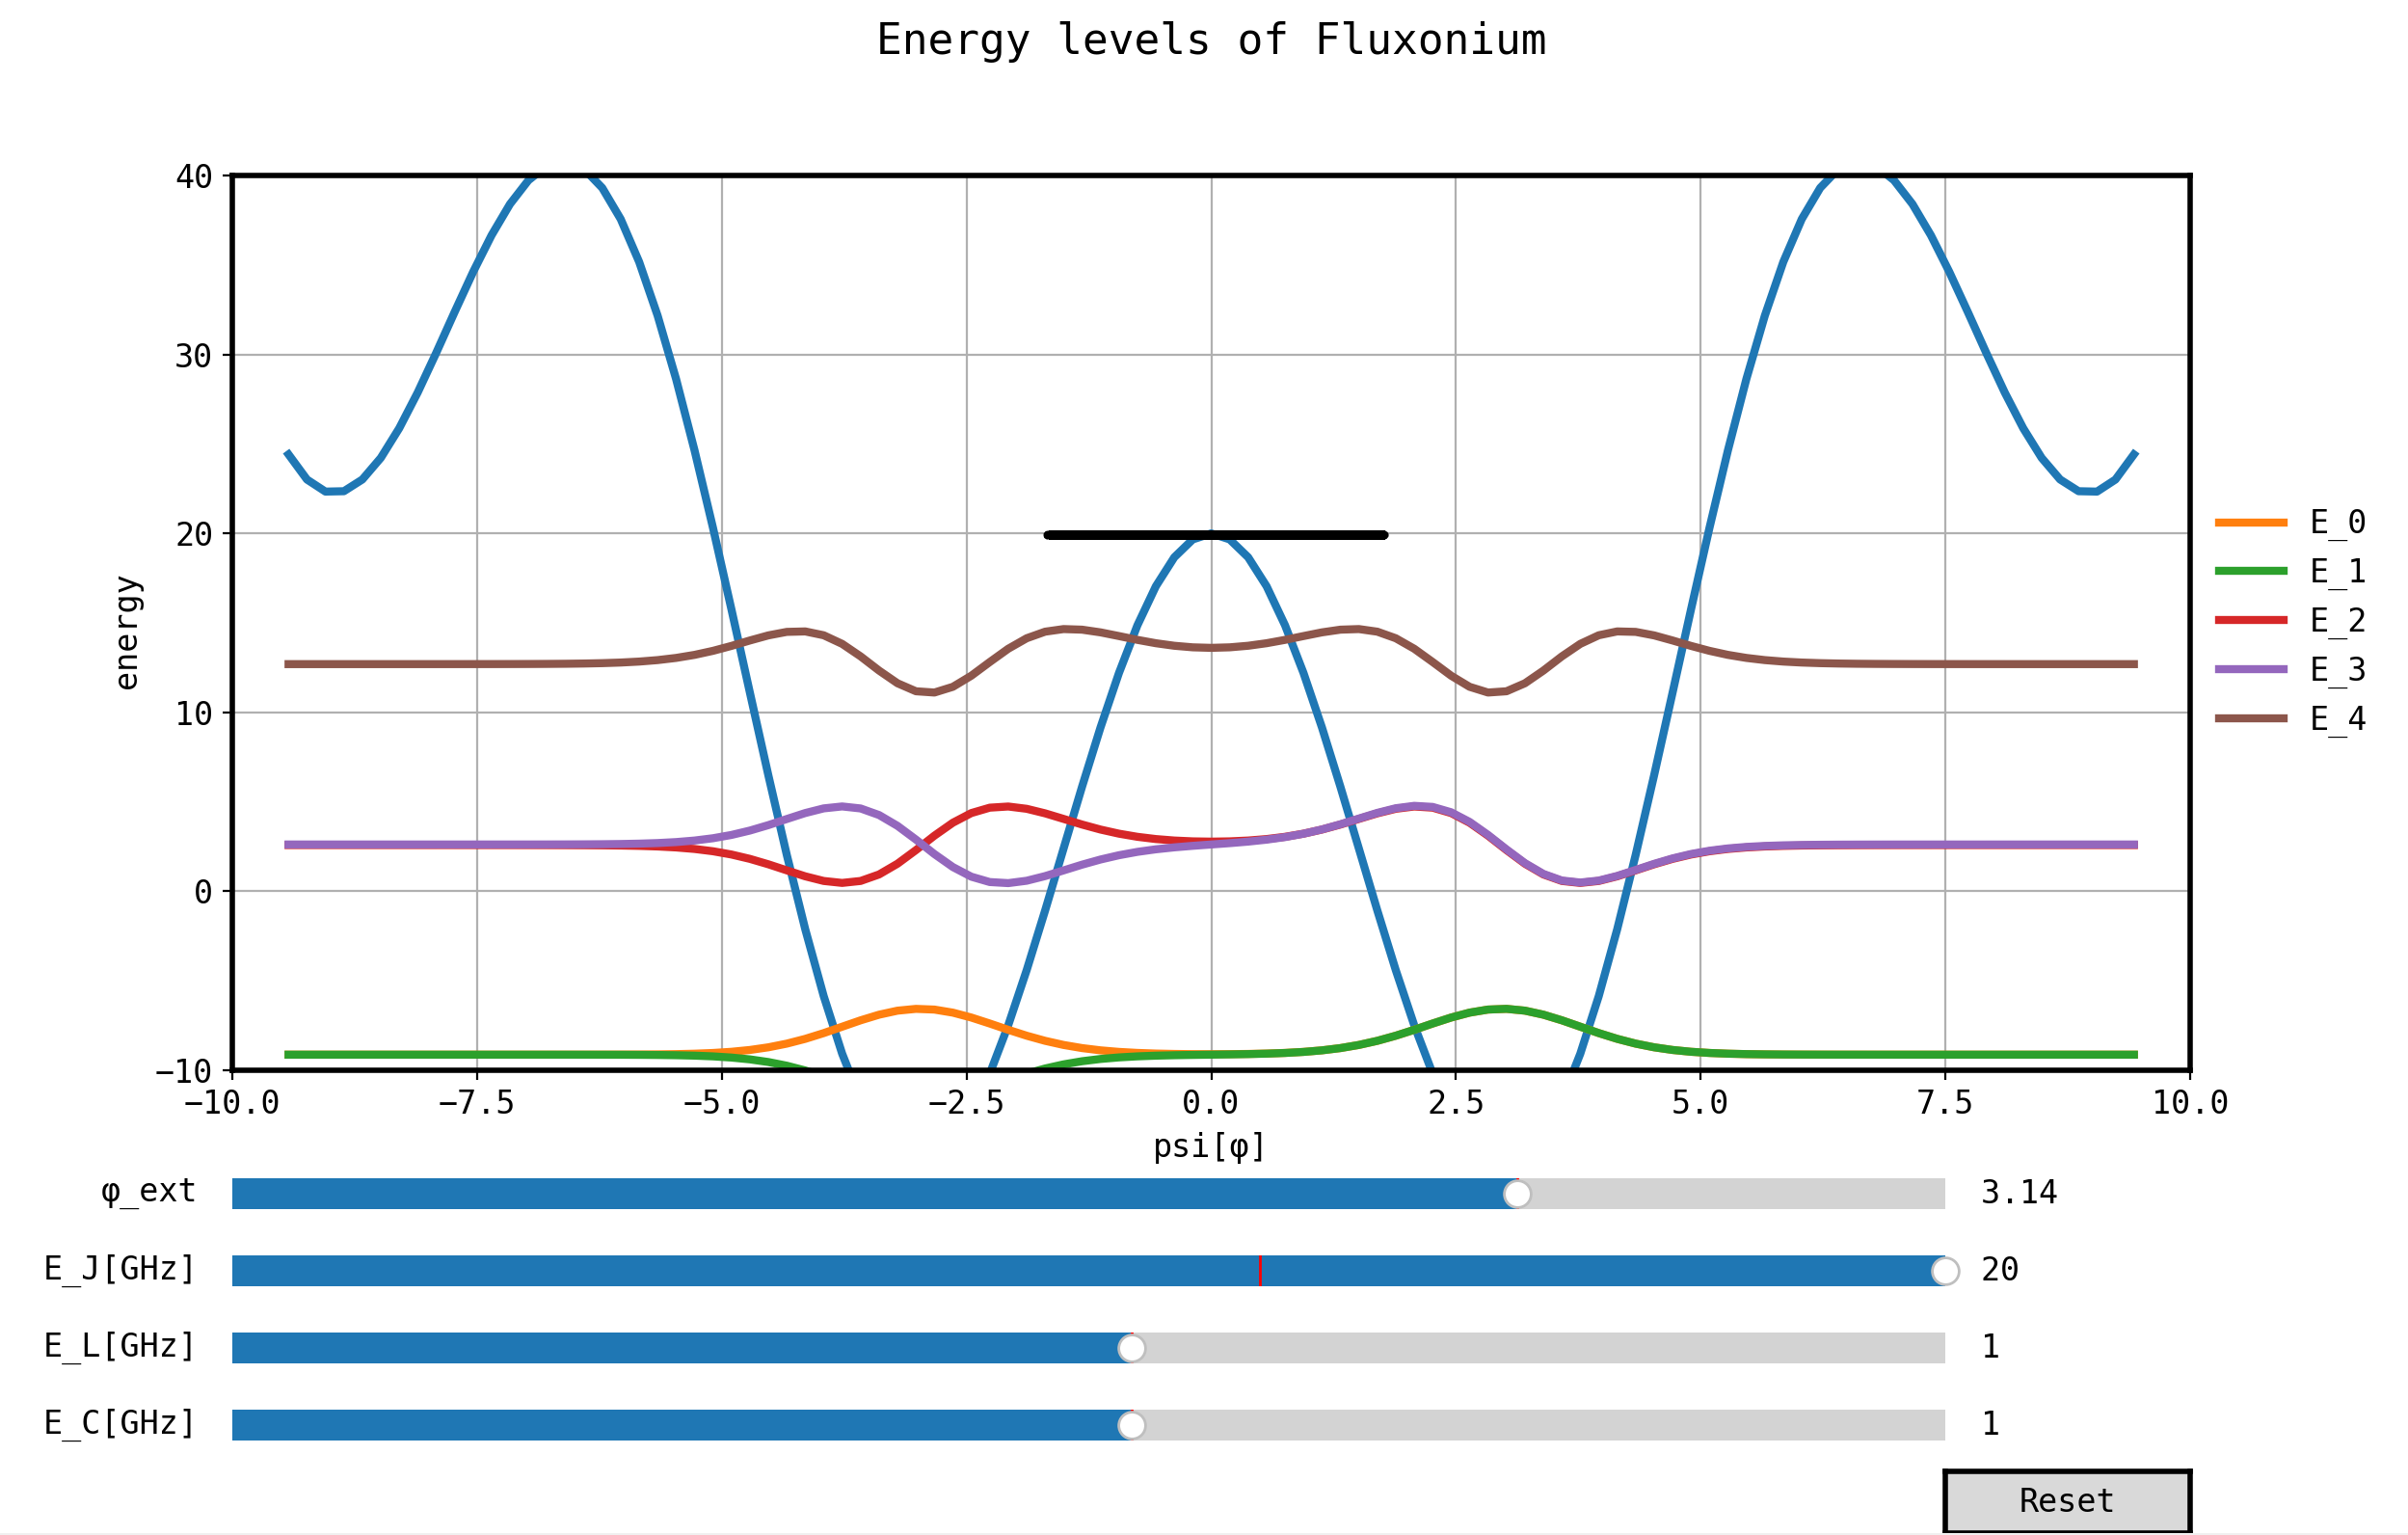
\includegraphics[width = 13.5cm]{Images/Wavefunctions_and_eigenstates_Fluxonium_large_EJ.png}
        \caption[Energy diagram of a Fluxonium qubit large ratio between EJ and EL]{\textbf{Energy diagram of a Fluxonium qubit large ratio between EJ and EL:} Snapshot of Fluxonium energy spectrum simulation as a function of phase, $\phi$. The external flux are $\phi_{ext} = \pi$, the capacitor energy, $E_C= 1$, the Jospehson energy, $E_J = 20$ and the inductance energy, $E_L = 1$ values. The black line indicate the potential between the 2 first energy levels.}
        \label{fig:Large_ratio_EJ_EL}
    \end{figure}

    \section{Conclusion on this section}
    This small "theoretical" project has grasped upon some theory behind superconducting qubits. I focused on the mean field \acrshort{bcs} theory and how it is used to described cooper pairs and Josephson junctions. Further, cavity QED was used as formalism to describe the superconducting circuits and derive an expression for the Hamiltonian in order to find eigen energies and eigen values of the Fluxonium circuit. Then, a numerical simulation of the Fluxonium qubit in the flux-basis was performed in order to find the optimal ratios between $\varphi_{ext}, E_C, E_J, and E_J$ to use for a Fluxonium qubit. When making a Fluxonium qubit you want that the two lowest energy levels, $E_1$ and $E_2$, are well defined and close in energy. Further you want a large anharmonicity between $\hbar \omega_{10}$ and $\hbar \omega_{21}$. This can be obtained by setting $\phi_{ext} = \pi$, $E_C $ to around 4, and having a large (but not too large) ratio between $E_J$ and $E_L$.


\chapter{Simulations of Energy level of Newfluxonium in python}
    
% \chapter{Simulations of Energy levels with noise and errors}
% \chapter{Simulations of 1 and 2 qubit gates}

\chapter{Simulation of Fluxonium circuit design in Ansys}
    
\chapter{Simulation of Newfluxonium circuit design in Ansys}